\documentclass[a4paper]{article}
\usepackage[T1]{fontenc}
\usepackage[utf8]{inputenc}
\usepackage[english]{babel}
\usepackage{frontespizio}
\usepackage{graphicx}
\usepackage{listings}
\usepackage{scrextend}
\usepackage[margin=1.2in]{geometry}
\usepackage[font=small,labelfont=bf]{caption}

\begin{document}
\selectlanguage{english}
\baselineskip 13pt
	
% ---- FRONTESPIZIO ----- 
\begin{frontespizio} 
 \Preambolo{\renewcommand{\frontpretitlefont}{\fontsize{15}{12}\scshape}}
\Istituzione {University of Pisa}
\Divisione {Scuola di Ingegneria}
\Corso [Laurea]{Artificial Intelligence and Data Engineering}
\Annoaccademico {2019--2020}
\Titolo { \vspace {35mm}Task3 Documentation}
\Filigrana [height=4cm,before=0.28,after=1]{./images/stemma_unipi.png}
\Rientro {1cm}
\Candidato {Alice Nannini}
\Candidato {Giacomo Mantovani}
\Candidato {Marco Parola}
\Candidato {Stefano Poleggi}
\Relatore {Prof. Pietro Ducange}
 \Punteggiatura {}
\end{frontespizio}


% ----- INDICE -----
\tableofcontents\thispagestyle{empty}
\clearpage


\section{Introduction}\pagenumbering{arabic}
This is an application to browse and evaluate university courses, called \textbf{Student-Evaluation}.\\
The application is developed to allow students (users) to view all the courses of a specific university with related comments.\\ 
Looking the table on the right side, a user can browse all subjects and by clicking an element of this table, on the left section, the user can see more information about the chosen element: general information and comments.\\ 
In order to filter the list of subjects, there is a choice box, thanks to which the user can select a specific degree course. \\
In order to leave a comment, it is necessary to log in, otherwise, the application will allow interaction in read-only.\\
There are two buttons in the bottom left corner to allow students to update or delete their comments. There is another button that allows a user to search students from a suggested list.


\begin{minipage}{\linewidth}
\begin{center}
\vspace{8mm}
\includegraphics[width=\textwidth]{./images/diagrams/Mockup.pdf} 
\vspace{3mm}
\captionof{figure}{Mockup}
\label{fig:mockup}
\end{center}
\end{minipage}

\clearpage

\section{Analysis and workflow}

% ----- REQUIREMENTS -----
\subsection{Requirements}

\subsubsection{Functional requirements}
The system has to allow the guest to carry out basic functions such as:
\begin{itemize}
\item To select a course from the list and view information and comments.
\item To select a degree course from the list, filtering subjects.
\end{itemize}
In addiction to the guest functions, the system has to allow the user to carry out basic functions such as:
\begin{itemize}
\item To login to the system.
\item To upload comments on a course.
\item To update a comment of a course only if the user is the owner.
\item To delete a comment of a course only if the user is the owner.
\item To add a friend.
\end{itemize}
\vspace{2mm}
The system has to allow the administrator to carry out basic functions such as:
\begin{itemize}
\item To login to the system.
\item To add a course.
\item To update a course.
\item To delete a course.
\item To add a professor.
\item To update a professor.
\item To delete a professor.
\item To associate a professor to a course.
\item To delete any comment.
\end{itemize}
\vspace{2mm}

\subsubsection{Non-functional requirements}
\begin{itemize}
\item Usability, ease of use and intuitiveness of the application by the user.
\item The system should provide access to the database with a few seconds of latency.
\end{itemize}

\clearpage

% ----- USE CASES -----
\subsection{Use cases}

\textbf{Actors}
\begin{itemize}
\item{Guest : this actor represents a user who is not logged into the system}
\item{Student : this actor represents a user who is logged into the system}
\item{Admin : this actor represents the administrator of the system}
\end{itemize}

\subsubsection{Use Cases Description}
\begin{table}[h]
\centering
\begin{tabular}{p{0.25\textwidth}p{0.25\textwidth}p{0.1\textwidth}p{0.4\textwidth}}
\hline
\textbf{Event} & \textbf{UseCase} & \textbf{Actor(s)} & \textbf{Description}\\ \hline

Log in, Log out & Login,  Logout & Admin, Student & The user logs in/out the application. The system browses the subjects' list by the degree course of the logged user and returns it on the interface.\\ \hline

View all the subjects & Browse, Find, Display Subject & Admin, Student, Guest & The user chooses that he wants to view the list of all subjects. The system browses the data on the db and returns them on the interface.\\ \hline

View the comments of a subject & Browse, Find, View Comment & Admin, Student, Guest & The user clicks on a record of the subject table. The system browses on the db the comments related to that subject and returns them on the interface.\\ \hline

Add a comment & Add Comment & Admin, Student & The user submits the text of his comment. The system updates the db and the interface.\\ \hline

Update a comment & Update Comment & Student & The user selects the comment and commits the new text. The system updates the db and the interface.\\ \hline

Delete a comment & Delete Comment & Admin, Student & The user selects the comment and submits the delete. The system updates the db and the interface.\\ \hline

View degree courses & Browse, Find, Display Degree & Admin, Student, Guest & The system browses the degree courses list and returns them on the interface.\\ \hline

Add a professor or a subject & Add Professor/Subject & Admin & The admin submits the name and other information of the new subject/professor. The system updates the db and the interface.\\ \hline

Update a professor or a subject & Update Prof/Subject & Admin & The user selects the subject/professor and commits the new information. The system updates the db and the interface.\\ \hline

Delete a professor or a subject & Delete Prof/Subject & Admin & The user selects the subject/professor and submits the delete. The system updates the db and the interface.\\ \hline

View suggested friends & Browse, Find, Display Student & Student, Admin & The user chooses that he wants to view the suggested friends. The system browses on the db the students and returns them on the interface.\\ \hline

Set find parameter & By Degree, By Subject & Admin, Student, Guest & The user chooses the filter to apply to the query on the database. The system uses it to find the results.\\ \hline

\end{tabular}
\end{table}

\begin{minipage}{\linewidth}
\begin{center}
\vspace{8mm}
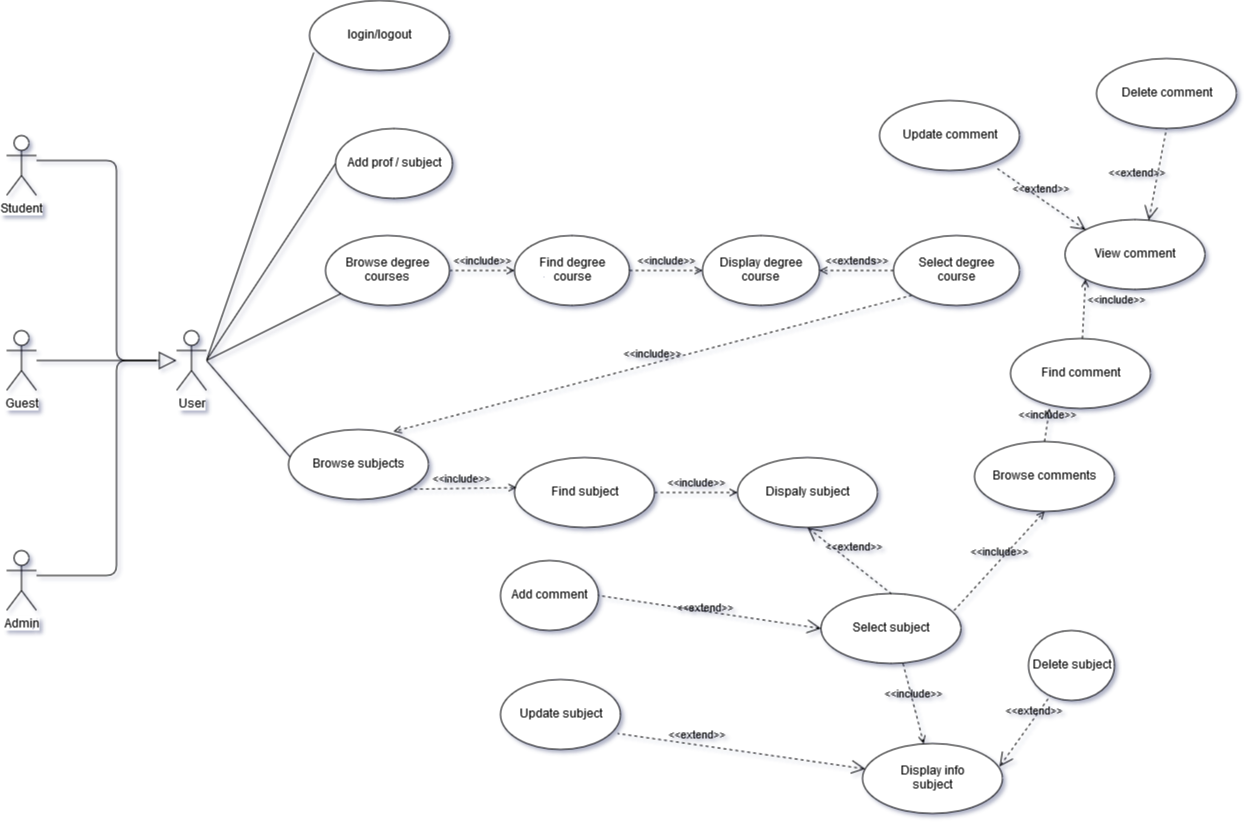
\includegraphics[height=11cm]{./images/diagrams/UseCases} 
\captionof{figure}{Use cases diagram}
\vspace{3mm}
\end{center}
\end{minipage}

\clearpage

\subsection{Analysis of entities}
This diagram represents the main entities of the application and the relations between them.
\begin{minipage}{\linewidth}
\begin{center}
\vspace{4mm}
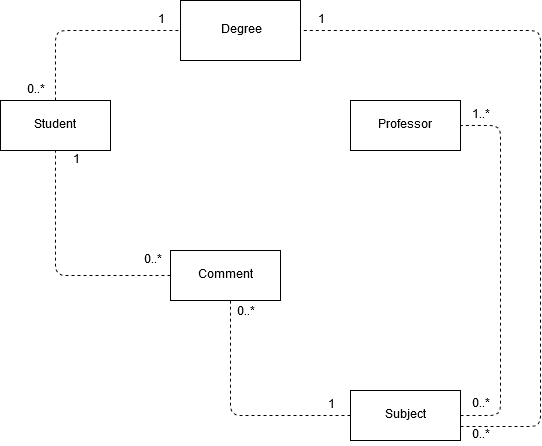
\includegraphics[width = 0.7\textwidth]{./images/diagrams/AnalysisUML.png} 
\vspace{2mm}
\captionof{figure}{UML analysis diagram}
\label{fig:analisys_diagram}
\end{center}
\end{minipage}

\clearpage
% ----- DESIGN -----
\section{Design}

% ----- DATABASE -----
\subsection{Database Choice}
This application is based on many join operations between the entities, in order to obtain each professor associated with a subject, or each comment associated with a subject, or yet display all the subjects associated with a degree course. For this reason, if the amount of data available is very high as expected, a relational database will be computationally expensive. Then the choice fell on a graph database, which manage to work very well and very fast on a model made with a lot of entities and relations. Moreover, a graph database is very useful for some specific queries in the application, for example, showing a suggested friends list. \\

% ----- ARCHITECTURE -----
\subsection{Software Architecture}
The application is designed over 2 different layers, see figure \ref{fig:architecture_diagram}:
\begin{itemize}
\item Front-end
\item Back-end
\end{itemize}
\begin{figure}[h]
\centering
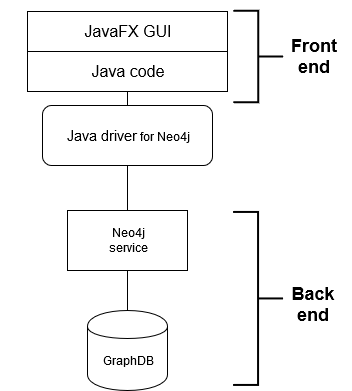
\includegraphics[width=0.4\textwidth]{./images/diagrams/architecture_diagram.png} 
\caption{Software architecture diagram\\}
\label{fig:architecture_diagram}
\end{figure}

% ----- GRAPH MODEL -----
\subsection{Structure of the database}
In graph databases the entities are modeling using the vertexes; in our model there are the following entities:
\begin{itemize}
\item Professor
\item Student
\item Degree
\item Subject
\item Comment
\end{itemize}
Moreover the relations are modeling using the edges; in our model there are the following edges:
\begin{itemize}
\item ATTENDS, which connects a student to a degree
\item TEACHES, which connects a professor to a subject
\item BELONGS, which connects a subject to a degree
\item WROTE, which connects a student to a comment
\item KNOWS, which connects a student to a student
\end{itemize}


\begin{minipage}{\linewidth}
\begin{center}
\vspace{4mm}
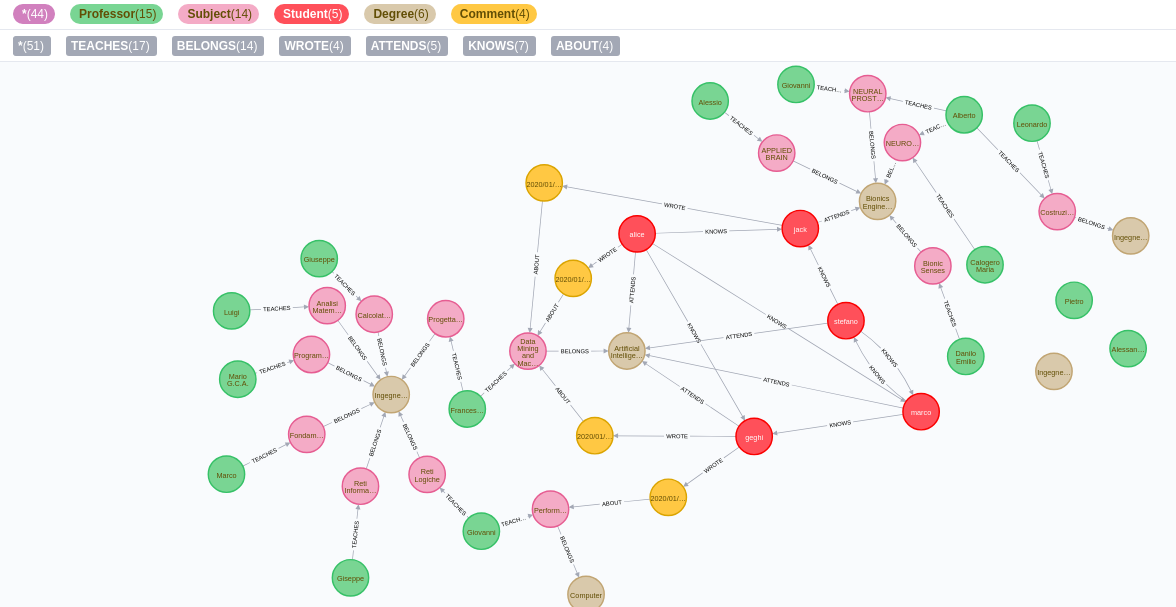
\includegraphics[width = 1\textwidth]{./images/diagrams/graphDb.png} 
\vspace{2mm}
\captionof{figure}{Graph model}
\label{fig:analisys_diagram}
\end{center}
\end{minipage}

% ----- GRAPH CENTRIC QUERY ------
\subsection{Query centric}
In order to make the most of the graph database's potential, we implement some functionality using query centric:
\begin{itemize}
\item To suggest friends
\item To retrieve comments of friends
\end{itemize}

\subsubsection{Suggestions of friends}
The following query is used to propose new friends to the logged user, it returns all Student vertexes for exists a path between two and four hope, in each directions. 
\begin{verbatim}
  MATCH (friend:Student)-[*2..4]-(s:Student) 
  WHERE ID(s) = $userId AND  
  NOT (s)-[:KNOWS]-(friend)  AND
  NOT ID(friend) = ID(s) 
  RETURN DISTINCT ID(friend), friend.username, friend.admin;
\end{verbatim}

\subsubsection{Retrieving comments}
The following query retrieves all the comment related to a subject, written by the friends of the logged user.\\
Please note that do this operation over a graph database is much more efficient than e relational database, in which we should compute a join operation involving 5 tables.
\begin{verbatim}
  MATCH (user:Student)-[:KNOWS]-> 
  (st:Student)-[:WROTE]->  
  (c:Comment)-[:ABOUT]->(s:Subject)  
  WHERE id(s) = $idSubject  
  AND id(user) = $idUser  
  RETURN ID(c),c.text,c.date,ID(st),st.username;
\end{verbatim}
\clearpage
% ----- IMPLEMENTATION -----
\section{Implementation}

\subsection{Used Technologies}
The application is developed in java programming language, version 11.0.4, and in JavaFX system to create the GUI, version 11, so it should run on each platform in which JVM is installed, but the application is tested and guardantee on Ubuntu 16 and Window OS. Moreover Maven is used  to build and mantain the project, version 3.8.0. \\
The java driver for Neo4j manages the comunication between the client application layer and the database backend layer, version 3.2.1.\\ 
For the backend layer it is used a graph database: Neo4j, version 3.2.1.\\
So this application is tested using these technologies, considering these particular versions: for other versions the correct execution isn't guaranteed .

% ----- CODE -----
\subsection{Java Classes Description}

In this section are listed the classes who model the entities.
\begin{itemize}
\item Student
\item Professor
\item Subject
\item Comment
\item Degree
\end{itemize}
Each of them have some attributes and the related Get and Set methods.

\subsubsection{Declaration of Student class}
\begin{verbatim}
public class Student{
    private final SimpleIntegerProperty id;
    private final SimpleBooleanProperty admin;
    private final SimpleStringProperty username;
    private final SimpleObjectProperty<Degree> degree;
    private final SimpleListProperty<Student> friends;
    
    // CONSTRUCTOR
    public Student(int i, String u, Degree d, boolean a) {
        id = new SimpleIntegerProperty(i);
        admin = new SimpleBooleanProperty(a);
        username = new SimpleStringProperty(u);
        degree = new SimpleObjectProperty<Degree>(d);
        friends = new SimpleListProperty<Student>(null);
    }
    //GETTERS AND SETTERS
    ...
}
\end{verbatim}

\subsubsection{Declaration of Subject class}
\begin{verbatim}
public class Subject {
    private final SimpleIntegerProperty id;
    private final SimpleStringProperty name;
    private final SimpleIntegerProperty credits;
    private final SimpleStringProperty info;
    private final SimpleIntegerProperty degree;
    private final SimpleListProperty<Professor> professors;
	
    // CONSTRUCTOR
    public Subject(int i, String n, int c, String inf, int d) {
        id = new SimpleIntegerProperty(i);
        name = new SimpleStringProperty(n);
        credits = new SimpleIntegerProperty(c);
        info = new SimpleStringProperty(inf);
        degree = new SimpleIntegerProperty(d);
        professors = new SimpleListProperty<Professor>(null);
    }
    ...
}
\end{verbatim}

\subsubsection{Declaration of Professor class}
\begin{verbatim}
public class Professor{
    private final SimpleIntegerProperty id;
    private final SimpleStringProperty name;
    private final SimpleStringProperty surname;
	
    // CONSTRUCTOR
    public Professor(int i, String n, String s) {
        name = new SimpleStringProperty(n);
        surname = new SimpleStringProperty(s);
        id = new SimpleIntegerProperty(i);
    }
    ...
}
\end{verbatim}

\subsubsection{Declaration of Degree class}
\begin{verbatim}
public class Degree {
    private final SimpleIntegerProperty id;
    private final SimpleStringProperty name;
    
    public Degree(int i, String n) {
        id = new SimpleIntegerProperty(i);
        name = new SimpleStringProperty(n);
    }
    ...
}
\end{verbatim}

\subsubsection{Declaration of Comment class}
\begin{verbatim}
public class Comment{

    private final SimpleIntegerProperty id;
    private final SimpleStringProperty text;
    private final SimpleIntegerProperty student;
    private final SimpleStringProperty date;
    private final SimpleIntegerProperty subject;

    public Comment(int i, String t, int s, int sub, String d) {
        id = new SimpleIntegerProperty(i);
        text = new SimpleStringProperty(t);
        student = new SimpleIntegerProperty(s);
        date = new SimpleStringProperty(d);
        subject = new SimpleIntegerProperty(sub);
    }
	...
}
\end{verbatim}

\subsubsection{Database manager}
The other important class in the project is the DbManager. It handles the connection with Neo4j and provides all methods to interact with it.

\begin{verbatim}
  public class DbManager implements AutoCloseable {
       private final Driver driver;
       private final String uri = "bolt://localhost:7687";
       private final String user = "user";
       private final String password = "pwd";

       public DbManager() {
          driver = GraphDatabase.driver(uri, AuthTokens.basic(user, password));
       }

    // ... crud operations ...

       @Override
       public void close() throws Exception {
          driver.close();
       }
  }
\end{verbatim}


% ----- CRUD OPERATION ------
\subsection{CRUD operations}
All crud operations are implemented using the \textbf{Cypher query language}; it is a declarative graph query language that allows for expressive and efficient querying and updating of a property graph.


\subsubsection{Create}
This method of the DbManager class guarantees the creation of a comment. A new vertex is inserted on the graph and  is connected with a student node using an incoming edge called WROTE. Moreover it is connected with a subject node, using an outgoing edge called ABOUT.

\begin{verbatim}
public void createComment(String text, Student student, int subjectId) {
   try(Session session = driver.session()){
       session.writeTransaction( tx -> {
           tx.run( "MATCH (e:Student) WHERE id(e) = $idStudent " + 
                   "MATCH (s:Subject) WHERE id(s) = $idSubject " +
                   "CREATE " + 
                   "(a:Comment {text: $text, date: $date})," + 
                   "(e)-[:WROTE]->(a)," + 
                   "(a)-[:ABOUT]->(s);", 
             Values.parameters("idStudent",student.getId(),"idSubject",subjectId,"text",text,
                   "date",new SimpleDateFormat("yyyy/MM/dd HH:mm:ss").format(new Date())) );
           return null;
       });
   }
}
\end{verbatim}


\subsubsection{Read}
This method reads from the database all the degrees and inserts them in a list.

\begin{verbatim}
public List<Degree> getDegreeCourses() {
   try(Session session = driver.session()){
      return session.readTransaction( tx -> {
         List<Degree> list = new ArrayList<>();
         StatementResult sr = tx.run( "MATCH (dd:Degree) RETURN ID(dd), dd.name;");
			
         while(sr.hasNext()) {
            Record r = sr.next();
            list.add(new Degree(r.get("ID(dd)").asInt(),r.get("dd.name").asString()));
         }
         return list;
      });
   }
}
\end{verbatim}


\subsubsection{Update}
The following snippet of code shows how to execute an updating operation of an entity professor.
\begin{verbatim}
  public void updateProfessor(int profId, String name, String surname) {
     try(Session session = driver.session()){
        session.writeTransaction( tx -> {
           tx.run("MATCH (p:Professor) WHERE ID(p) = $profId\n" + 
                  "SET p.name = $name, p.surname = $surname;",
             Values.parameters("profId",profId,"name",name,"surname",surname) );
           return null;
        });
     }
  }
\end{verbatim}

\subsubsection{Delete}
This example of deleting operation shows how to remove a subject, given its id, and the related relations.

\begin{verbatim}
  public void deleteSubject(int subjectId) {
     try(Session session = driver.session()){
        session.writeTransaction( tx -> {
           tx.run( "MATCH (n:Subject) WHERE id(n) = $idSubject DETACH DELETE n;",
             Values.parameters("idSubject",subjectId));
           return null;
        });
     }
  }
\end{verbatim}
\clearpage
% ----- MANUAL -----
\section{User Manual}
When you first run the application, the interface you get is the one in figure~\ref{fig:screen0}. 

\begin{figure}[h]
\centering
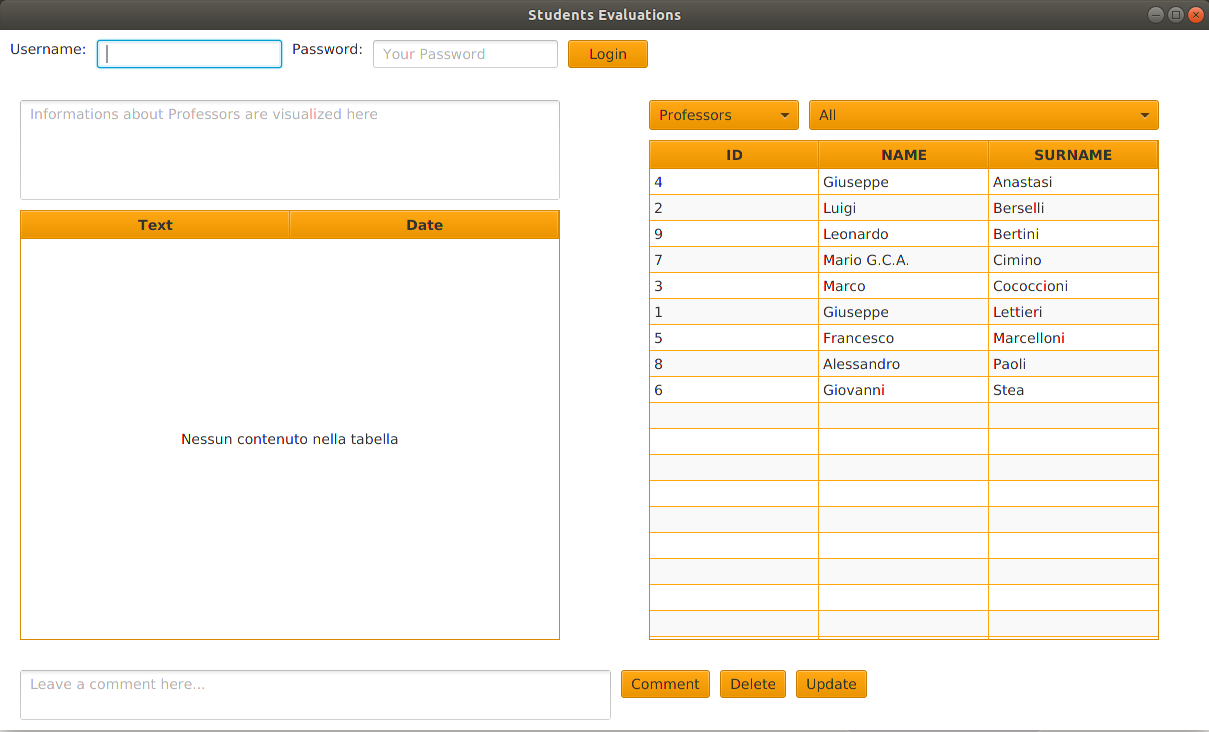
\includegraphics[width=0.88\textwidth]{images/screens/screen0}
\captionof{figure}{First view of the application}
\label{fig:screen0}
\end{figure}

The default display includes the list of all registered subjects in the table on the right. You can also choose to display the subjects of a single degree course, using the drop-down menu on the right (fig.~\ref{fig:screen1}).

\begin{figure}[h]
\centering
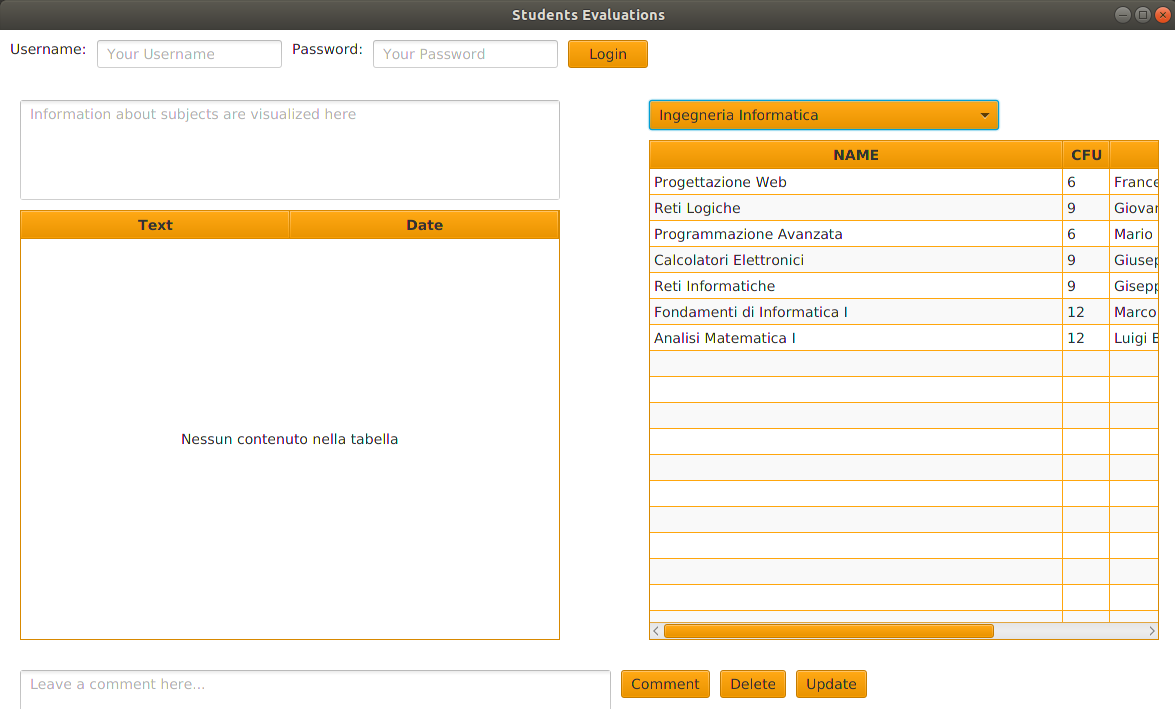
\includegraphics[width=0.88\textwidth]{images/screens/screen1}
\captionof{figure}{Selection of subjects filtered by the "Ingegneria Informatica" degree course}
\label{fig:screen1}
\end{figure}
\clearpage

If you have a registered account, you can log in to the application, so that the comments' operations aren't blocked. Enter your username and your password in the suited fields at the top and click on "Login" (fig.~\ref{fig:screenLogin}).
\begin{figure}[h]
\centering
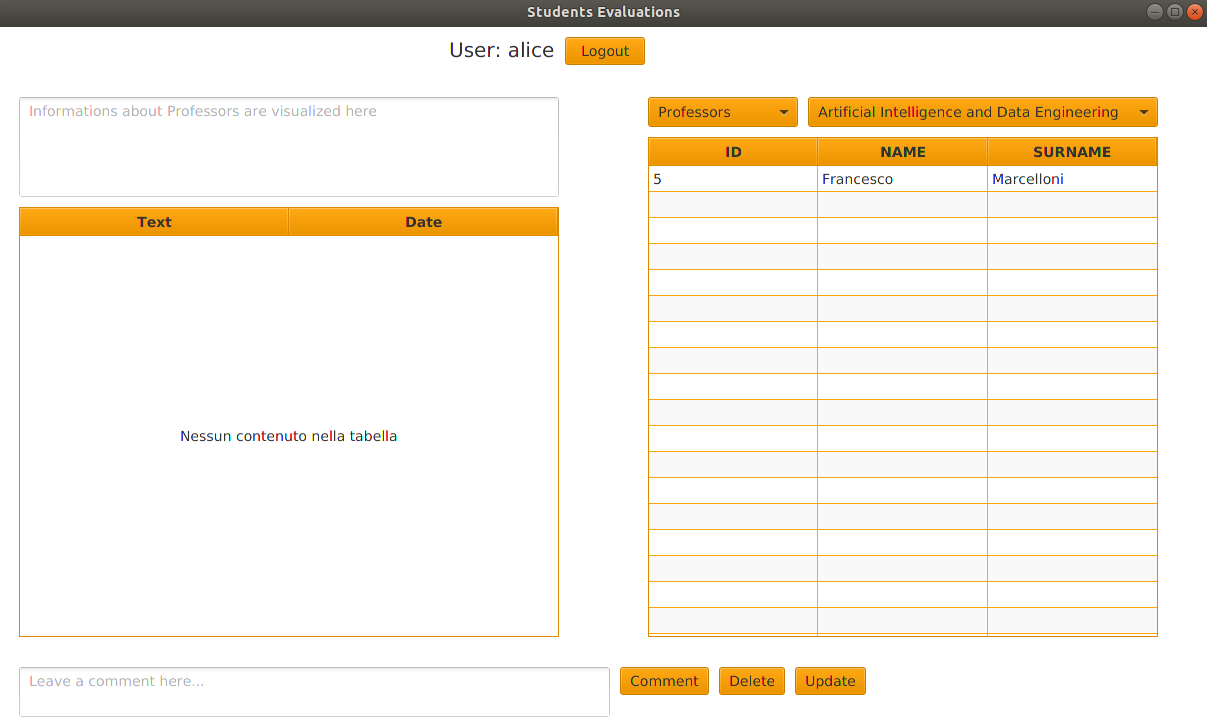
\includegraphics[width=0.88\textwidth]{images/screens/screenLogin}
\captionof{figure}{Application interface after the user "Alice" has logged in}
\label{fig:screenLogin}
\end{figure}

If you now want to be able to see the comments associated with a particular subject, you have to click on the name of the subject: in the table on the left the list of comments already received will appear (fig.~\ref{fig:screen3}). With this operation, you'll be able to visualize also the information related to that particular subject.

To leave a comment, you need to enter the text in the field below the table and then click on the "Comment" button. The result obtained from these operations is shown in fig.~\ref{fig:screen4}.

\begin{figure}
\centering
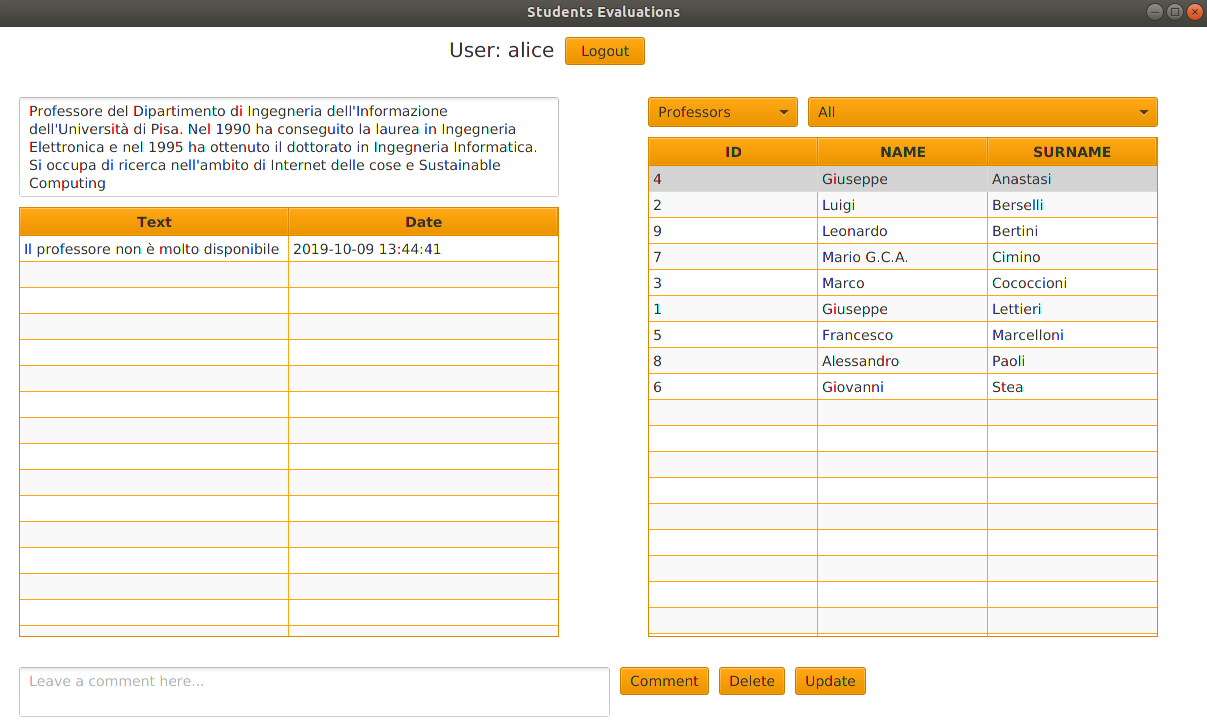
\includegraphics[width=0.9\textwidth]{images/screens/screen3}
\captionof{figure}{Displaying the comments related to a subject}
\label{fig:screen3}
\end{figure}

\begin{figure}
\centering
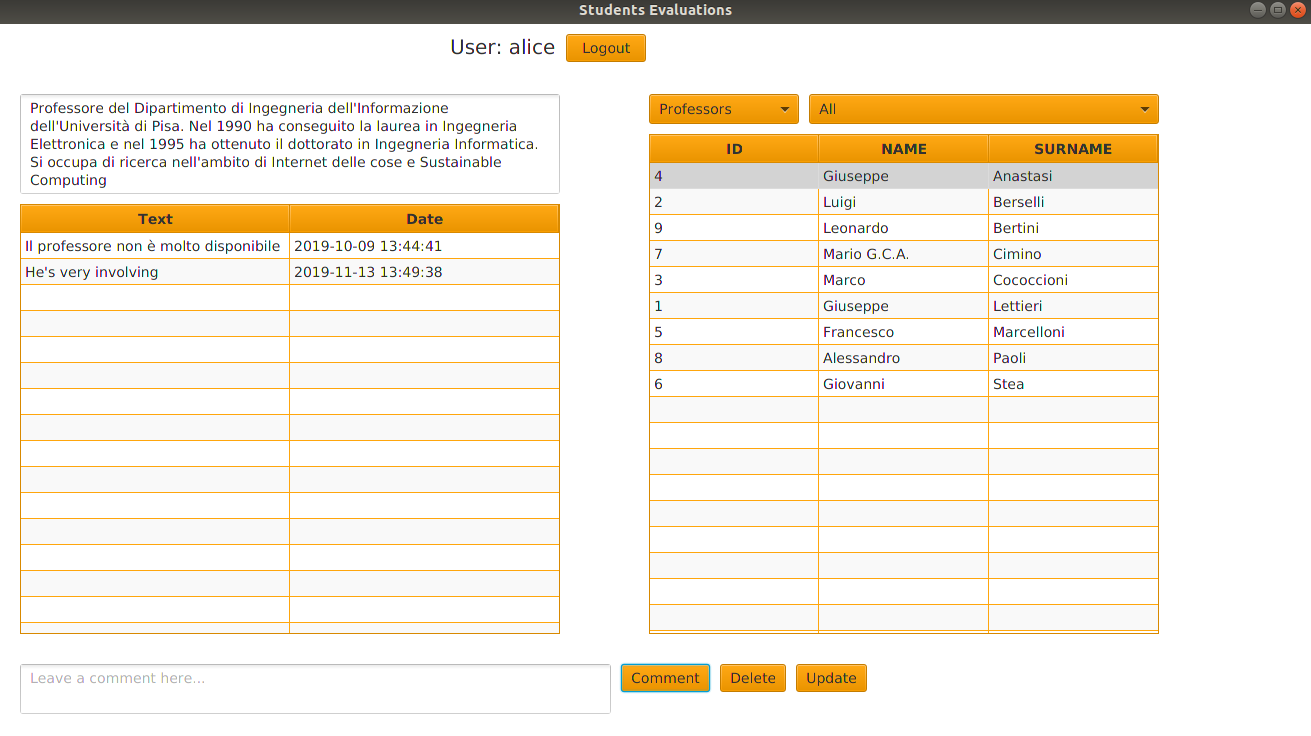
\includegraphics[width=0.9\textwidth]{images/screens/screen4}
\captionof{figure}{Interface after adding a comment}
\label{fig:screen4}
\end{figure}

You can also decide to modify the comment you just uploaded or another comment you made on a previous session. To do so, you need to click on the comment you want to update, change the text in the field below the table and then click on the "Update" button (fig.~\ref{fig:screen5}).
Finally you have the chance to delete your comment, by clicking on "Delete" after selecting it. Notice that you can modify or delete just the comments that you made.

\begin{figure}[h]
\centering
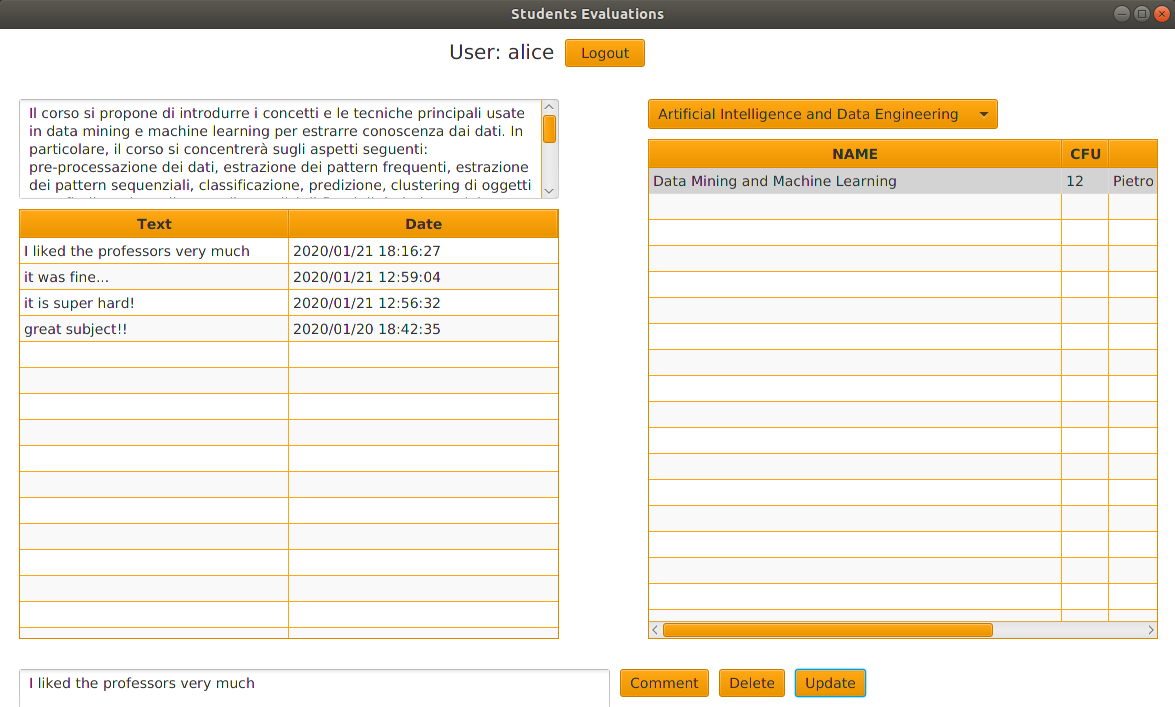
\includegraphics[width=0.88\textwidth]{images/screens/screen5}
\captionof{figure}{Interface after updating a comment}
\label{fig:screen5}
\end{figure}

To log out, just click on the appropriate button at the top, next to the user label.

Moreover, if you don't have a registered username, you can still browse through the application, search for subjects' information and read all comments. You are just unable to leave or change any comments.

\clearpage
%ADIMN MANUAL%
\subsection{Admin Manual}
If you have an admin user, you are entitled to make changes both on the professors' and the subjects' lists. You need to log in inserting your username and password, and the application will recognize you as the administrator and show up the buttons for modifying the data (fig.~\ref{fig:adminLogin}).

\begin{figure}[h]
\centering
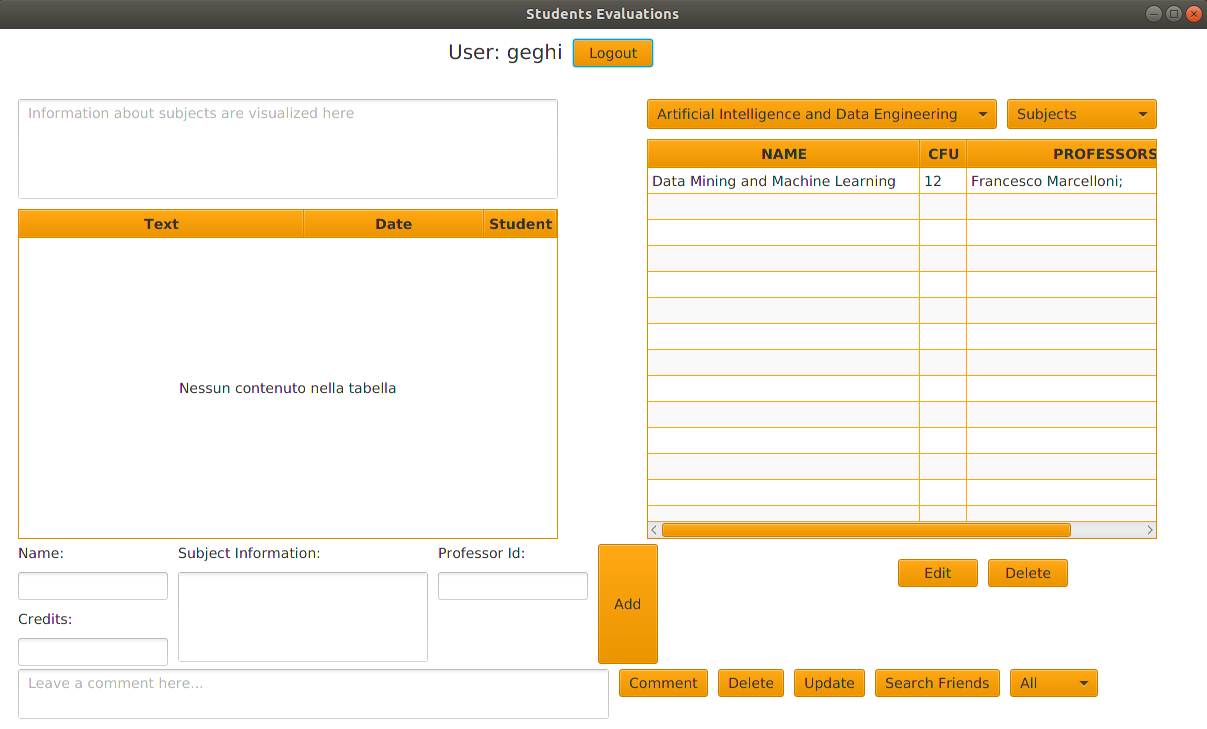
\includegraphics[width=0.88\textwidth]{images/screens/adminLogin}
\captionof{figure}{Interface after the administrator has logged in}
\label{fig:adminLogin}
\end{figure}
As an administrator, there's one extra table available, that you can view by choosing on the choice box appeared on the right (fig.~\ref{fig:admin0}). So you can see all the professors on the database and also adding new ones or updating the ones already in there.

\begin{figure}[h]
\centering
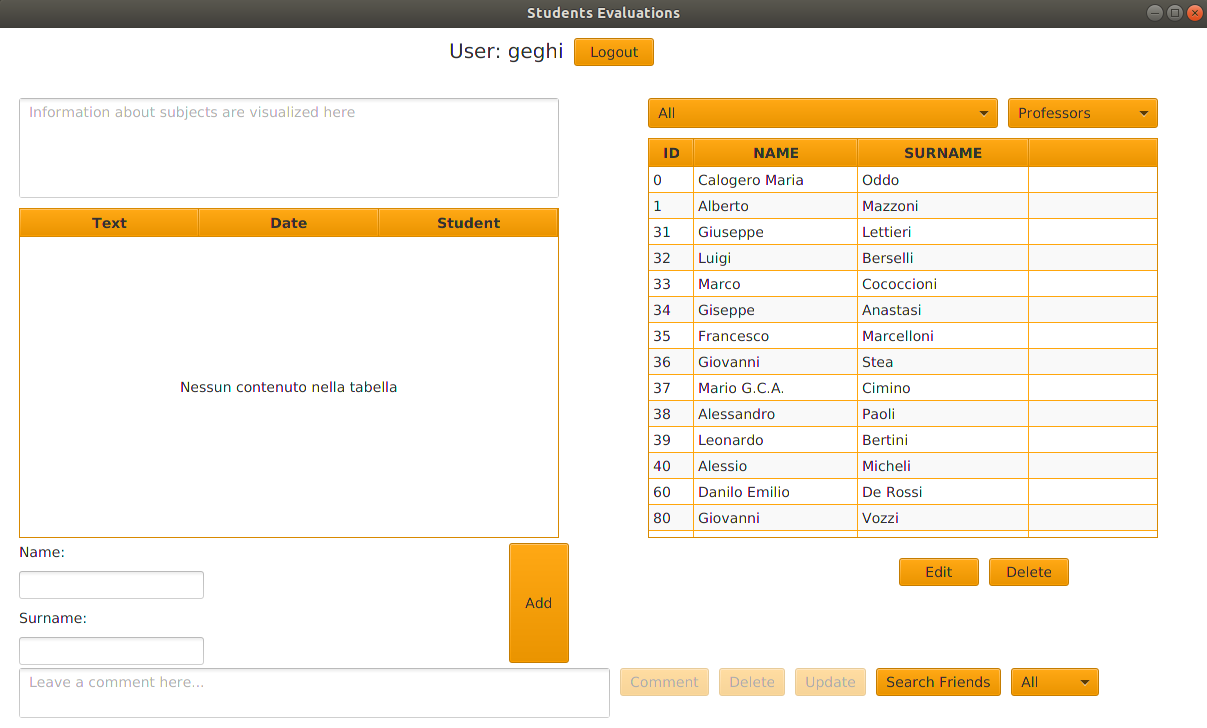
\includegraphics[width=0.88\textwidth]{images/screens/admin0}
\captionof{figure}{Displaying the professors' table }
\label{fig:admin0}
\end{figure}

You can choose to add a new professor, using the input fields at the bottom left. You have to specify the name and the surname, then press the "Add" button (fig.~\ref{fig:admin1}).
\begin{figure}[h]
\centering
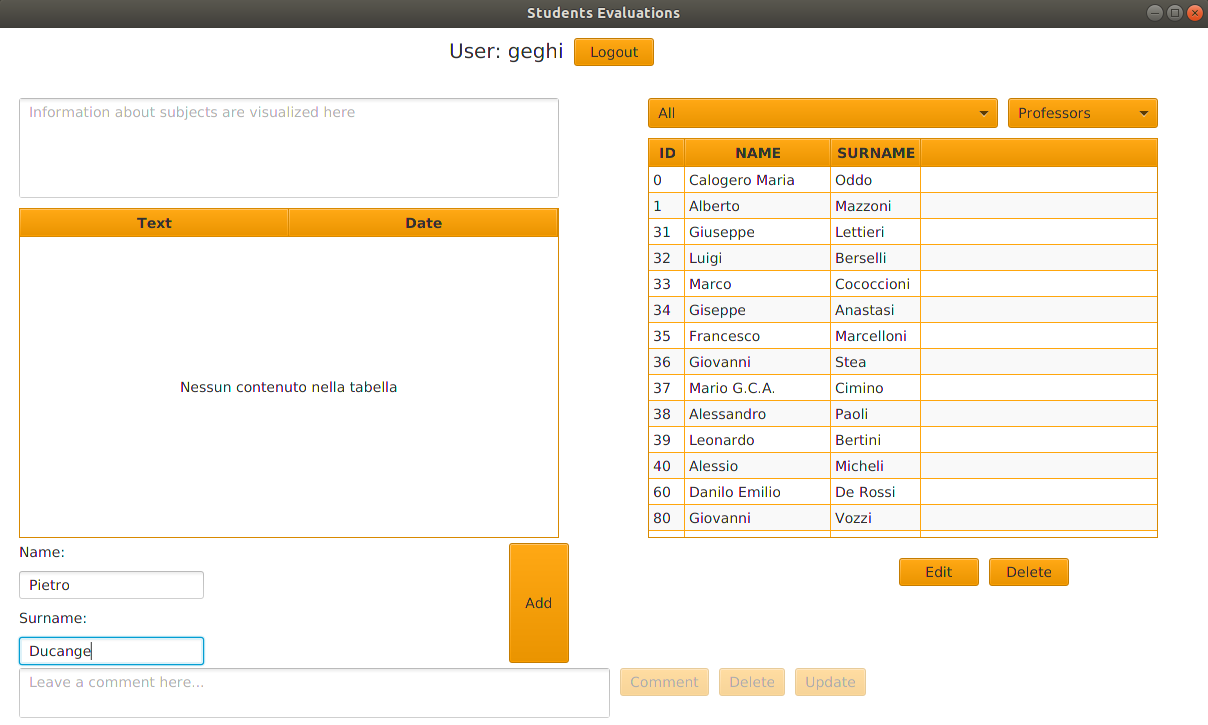
\includegraphics[width=0.88\textwidth]{images/screens/admin1}
\captionof{figure}{Adding a new professor}
\label{fig:admin1}
\end{figure}
\clearpage
You can also modify the data related to a professor: click on the professor you are interested in and change the information shown in the apposite input fields. Finally, you have the chance to delete a professor by clicking on the "Delete" button after selecting the wanted professor (fig.~\ref{fig:admin2}).
\begin{figure}[h]
\centering
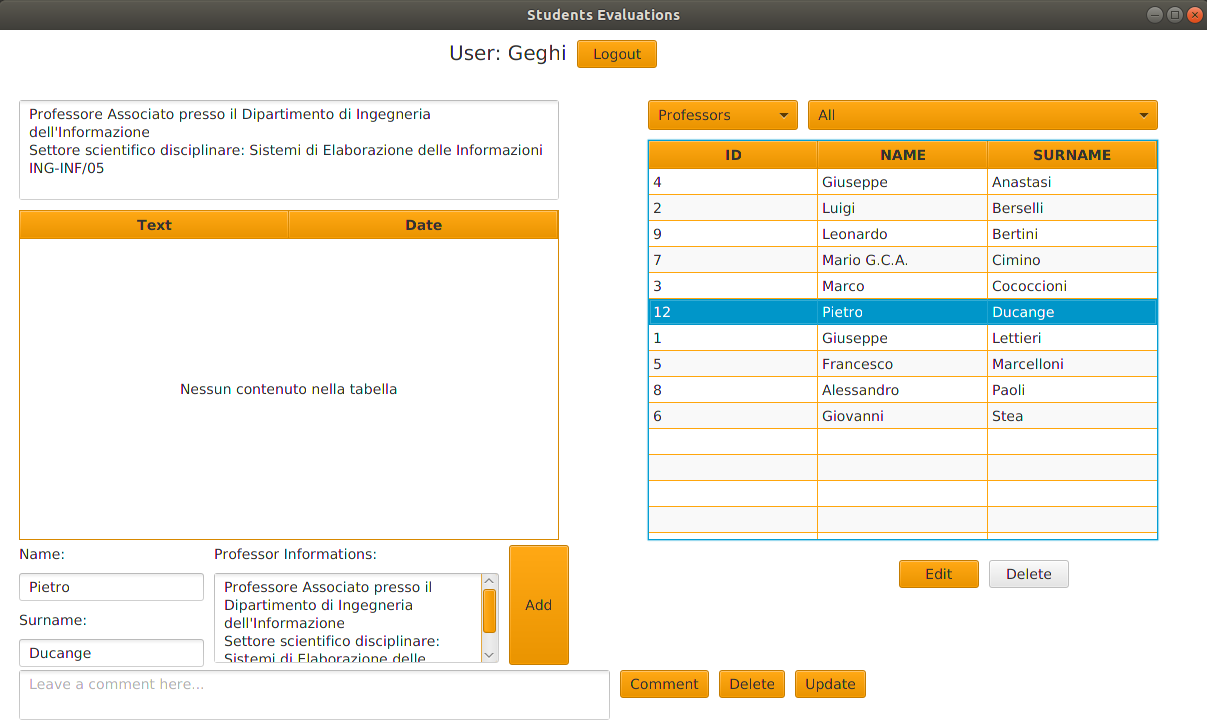
\includegraphics[width=0.88\textwidth]{images/screens/admin2}
\captionof{figure}{Screen of the application's interface from which you can either update or delete a professor}
\label{fig:admin2}
\end{figure}

All these operations are available for the subjects as well. The only difference is that when you want to add a new subject you also need to specify the id of the professor teaching it (or a list of ids, separeted by commas, if there are more professors teaching it). Moreover, you must have precisely displayed in the table the subjects of the same degree course of the new one (fig.~\ref{fig:admin3}).
\begin{figure}[h]
\centering
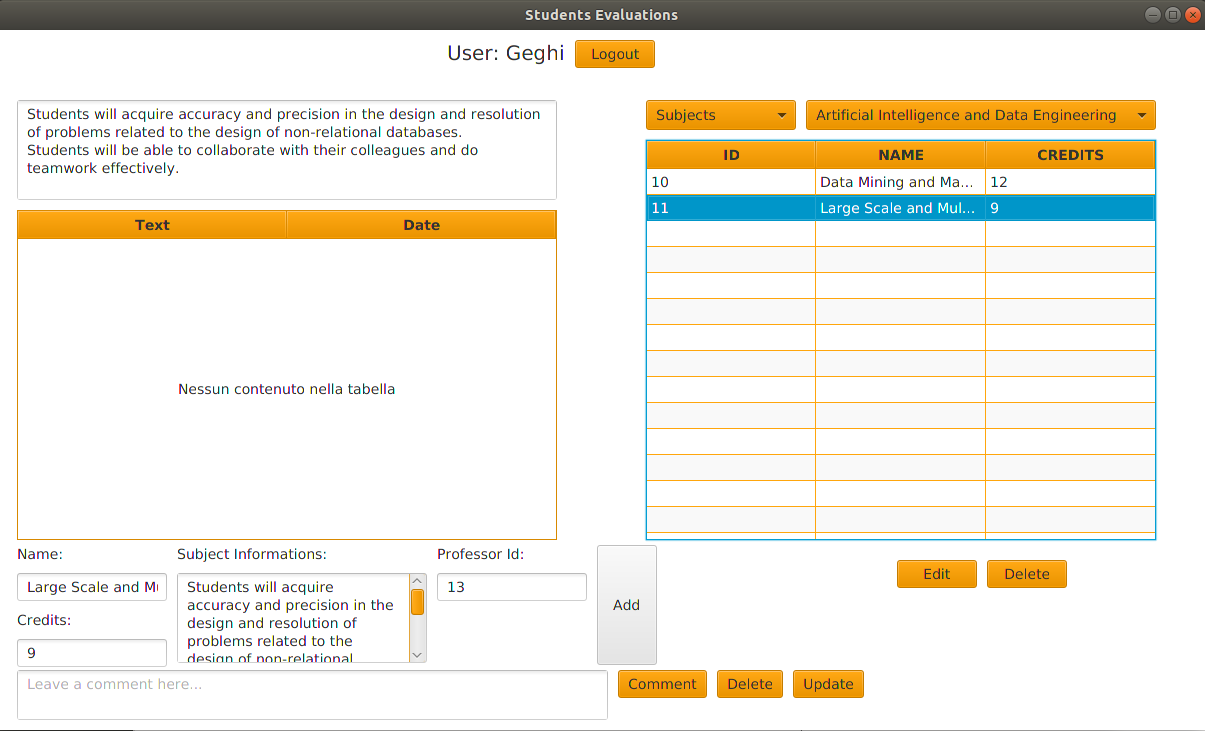
\includegraphics[width=0.88\textwidth]{images/screens/admin3}
\captionof{figure}{Interface after adding a new subject, ready to modify or delete it}
\label{fig:admin3}
\end{figure}
\clearpage
The administrator can delete comments posted by all the users, too. Just click on the comment and then on the "Delete" button (fig.~\ref{fig:admin4}).
\begin{figure}[h]
\centering
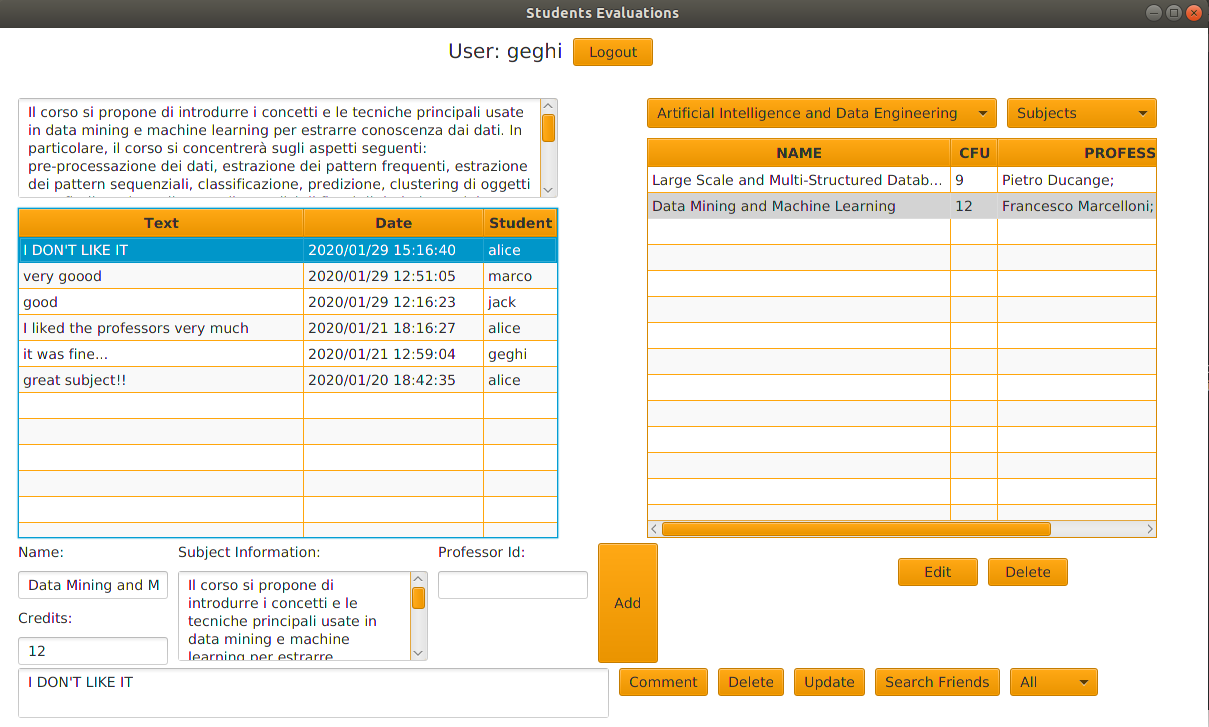
\includegraphics[width=0.88\textwidth]{images/screens/admin4}
\captionof{figure}{Screen of the application's interface from which the admin can delete a comment}
\label{fig:admin4}
\end{figure}


\end{document}